\documentclass{article}
\usepackage[margin=1in]{geometry}
\usepackage{amsmath}
\usepackage{amssymb}
\usepackage{bm}
\usepackage{pdfpages}
\usepackage{graphicx}
\usepackage{mathtools}
\usepackage{eurosym}
\usepackage[hidelinks]{hyperref}

\usepackage{fancyhdr}
\pagestyle{fancy}
\lhead{Ahou L. -  Ahou S. - Fiorini L. - Portier A.} % controls the left corner of the header
\chead{} % controls the center of the header
\rhead{Groupe 49} % controls the right corner of the header
\lfoot{} % controls the left corner of the footer
\cfoot{} % controls the center of the footer
\cfoot{~\thepage} % controls the right corner of the footer
\usepackage{titlesec}

% Commands for physic unit
\newcommand{\unit}[1]{[\mathrm{#1}]}

\begin{document}

\section*{Question 4A}
Puisque nous nous intéressons seulement aux bilans de productions/consommations et du niveau du bassin
sur des périodes de $T \unit{h}$, nous pouvons exprimer toutes nos variables en fonction de cette période.\\
Voici deux tableaux reprenant les notations principales utilisées dans cette seconde partie \footnote{Toutes autres notations utilisées dans la suite seront définies lorsque celles-ci seront introduites} : 

\begin{table}[h!]
    \centering
    \renewcommand{\arraystretch}{1.5}% Add spacing between rows : default value is 1
    \begin{tabular}{|c || c |} 
        \hline
        Nom & Signification\\
        \hline\hline
        $c_i$ & Capacité éolienne installée sur le i\textsuperscript{ème} site\\
        $t_j$ & Puissance à envoyer en turbinage choisie durant la j\textsuperscript{ème} période\\
        $p_j$ & Puissance de pompage choisie durant la j\textsuperscript{ème} période\\
        \hline
    \end{tabular}
    \caption{Table des notations des variables de décisions utilisées pour le modèle de la question 4.}
    \label{table:notations_variables_4}
\end{table}

\begin{table}[h!]
    \centering
    \renewcommand{\arraystretch}{1.5}% Add spacing between rows : default value is 1
    \begin{tabular}{|c || p{14cm} |} 
        \hline
        Nom & Signification\\
        \hline\hline
        $n$ & Nombre de sites éoliens \\
        $m$ & Nombre de périodes de $T \unit{h}$ dans une année\\
        $e_i(j)$ & Rendement éolien du i\textsuperscript{ème} site durant la j\textsuperscript{ème} période\\
        $a_j$ & Apport fluvial durant la j\textsuperscript{ème} période\\
        $\mathrm{cons}_j$ & Consommation énergétique durant la j\textsuperscript{ème} période\\
        $t_\mathrm{max}$ & Capacité maximale d'énergie générée par le turbinage (Sur une période de T heures)\\
        $p_\mathrm{max}$ & Capacité maximale de pompage (Sur une période de T heures)\\
        $\mathrm{stock}_\mathrm{max}$ & Capacité de stockage maximale\\
        $\eta$ & Rendement de turbinage\\
        $\mathrm{costs}$ & Vecteur donnant les valeurs du coût d'installation d'un site éolien  (onshore/offshore) \newline $\mathrm{costs}_i = $ Coût d'installation d'un site onshore si le site d'index $i$ est onshore, et inversement.\\  
        \hline
    \end{tabular}
    \caption{Table des notations des constantes utilisées pour le modèle.}
    \label{table:notations_constantes}
\end{table}

\noindent
Le modèle peut alors s'écrire ainsi :
\begin{align}
    \min_{c_{i},t_j,p_j} \quad &\mathrm{costs}^\intercal\mathbf{c} \nonumber\\
    \textrm{tel que} \quad & \sum_{i=0}^{n-1} c_i e_i(j) + \eta \cdot t_j - p_j \ge \mathrm{cons}_j \quad \forall j \in  \{ 0, \ldots, m-1 \}\label{eq:4A_contr1}\\
    & 0 \le \frac{\mathrm{stock}_\mathrm{max}}{2}  + \sum_{j=0}^{k} p_j - t_j + a_j \le  \mathrm{stock}_\mathrm{max} \quad \forall k \in \{ 0, \ldots, m-2 \}\label{eq:4A_contr2}\\
    & \sum_{j=0}^{m-1} p_j - t_j + a_j = 0 \label{eq:4A_contr3}\\
    & 0 \le c_i \le c_i^\mathrm{max} \quad \forall i \in  \{ 0, \ldots, n-1 \}  \label{eq:4A_contr4}\\
    & 0 \le \eta \cdot t_j \le  t_\mathrm{max} \quad \forall j \in  \{ 0, \ldots, m-1 \}  \label{eq:4A_contr5}\\
    & 0 \le p_j \le  p_\mathrm{max} \quad \forall j \in  \{ 0, \ldots, m-1 \} \label{eq:4A_contr6}
\end{align}

\newpage

La fonction objectif représente le coût total d'installation des éoliennes (en tenant compte des différences entre les installations \textit{offshore} et \textit{onshore}). \\
La contrainte \eqref{eq:4A_contr2} fait le bilan lié aux variations des opérations de turbinage/pompage décidées et de l'apport fluvial naturel depuis le temps $t = 0$ jusqu'en tout temps $t = k$ afin de calculer l'augmentation/la diminution du niveau de l'eau dans le bassin.\\
La formalisation peut s'obtenir en sachant que le niveau initial de notre bassin est à $0.5 \times \mathrm{stock}_\mathrm{max}$, puis que le niveau du bassin au prochain temps est le niveau du bassin passé plus les fluctuations à la période $j$, pompage - turbinage + apport fluvial, qui est donné plus formellement par $\mathrm{bassin}_{j+1} = \mathrm{bassin}_{j} + p_j - t_j + a_j$, donc en développant cette relation de récurrence, nous obtenons 
bien le niveau de notre bassin pour toute période $j \in \{ 0, \ldots, m-1 \}$ en fonction de nos variables, et en sachant que le niveau du bassin doit revenir à son niveau initial, à la fin 
de la période considérée, il y a une contrainte "en moins" pour \eqref{eq:4A_contr2} qui apparaît dans \eqref{eq:4A_contr3}. \\
La contrainte \eqref{eq:4A_contr3} indique que le niveau final du bassin doit revenir au même niveau qu'initialement. Autrement dit, les opérations de turbinage/pompage et 
l'apport fluvial doivent se sommer à 0 à la fin de la dernière période.\\
Les contraintes \eqref{eq:4A_contr4}, \eqref{eq:4A_contr5} et \eqref{eq:4A_contr6} indiquent respectivement les bornes sur les capacités éoliennes maximales installables sur chaque site, 
les capacités maximales de turbinages et les capacités maximales de pompages pour des périodes de $T \unit{h}$, regroupées au niveau européen, bien entendu.
Nous avons cependant supposé pour la \eqref{eq:4A_contr5} contrainte, liée au turbinage, que la valeur $t_j$ est ce que 
nous extrayons du bassin, puis
la capacité $t_\mathrm{max}$ restreint alors l'énergie en sorte de la turbine($\eta \cdot t_j$), qui sert à la 
production électrique dans la condition \eqref{eq:4A_contr1}.

\newpage % Car il faudra rendre sur Gradescope en séparant les questions

\section*{Question 4B}
Suite à l'implémentation de notre problème d'optimisation sur le notebook Jupyter, nous obtenons 
un coût moyen qui est d'environ $\mathbf{58.282}$\euro/MWh. \footnote{C'est une valeur qui semble cohérente, surtout pour un modèle comme ici, 
assez libre et qui ne prétend pas refléter les réalités, le prix moyen de l'énergie par MWh en Europe actuellement 
est aux alentours de quelques centaines d'euros, d'après la Commission européenne : 
\url{https://ec.europa.eu/eurostat/statistics-explained/index.php?title=Electricity_price_statistics}, 
consulté le 8 mai 2024 à 01h08.} Nous avons implémenté ce problème avec la bibliothèque CVXPY qui a été recommandée, cependant
il y a plusieurs solvers disponibles et ils donnent pour ceux qui ont été testé, des résultats différents qui arrivent presque à
la même valeur de fonction objectif, la différence étant sûrement due aux erreurs de calcul numérique. Nous vous présentons des résultats 
en fonction des solvers étant relativement efficaces, bien qu'il y en ait plus pour la programmation linéaire. Pour cette résolution,
nous avons utilisé "PDLP" (la liste des solvers étant disponible ici : \url{https://www.cvxpy.org/tutorial/solvers/index.html}).

\begin{table}[h!]
    \centering
    \renewcommand{\arraystretch}{1.5}% Add spacing between rows : default value is 1
    \begin{tabular}{| c | c | c |} 
        \hline
        Solver & Temps de calcul & Coût total (Valeur de la fonction objectif) \\
        \hline
        PDLP & 3 minutes et 37.5 secondes & 150960698186.38720 \\
        SCIPY & 36.5 secondes & 150961169167.04733 \\
        \hline
    \end{tabular}
    \caption{Table comparative des solvers employés pour la résolution du modèle de la question 4 en fonction de leurs temps de calcul
    et du résultat renvoyé.}
    \label{table:comparaison_solver_Q4}
\end{table}
\noindent
Bien que SCIPY est plus rapide à nous fournir le résultat, nous trouvions que le choix des paramètres était moins bien représentable
graphiquement, mais cela aurait été une autre solution tout aussi efficace (à priori, en faisant l'hypothèse que les deux résultats de la fonction objectif 
sont sensiblement similaires). Nous n'avons pas fait de moyenne sur le temps de calcul mais 
ils semblent bien se comporter, il s'agit plus d'un ordre de grandeur que d'une valeur précise d'efficacité.


\begin{figure}[h!]
    \centering
    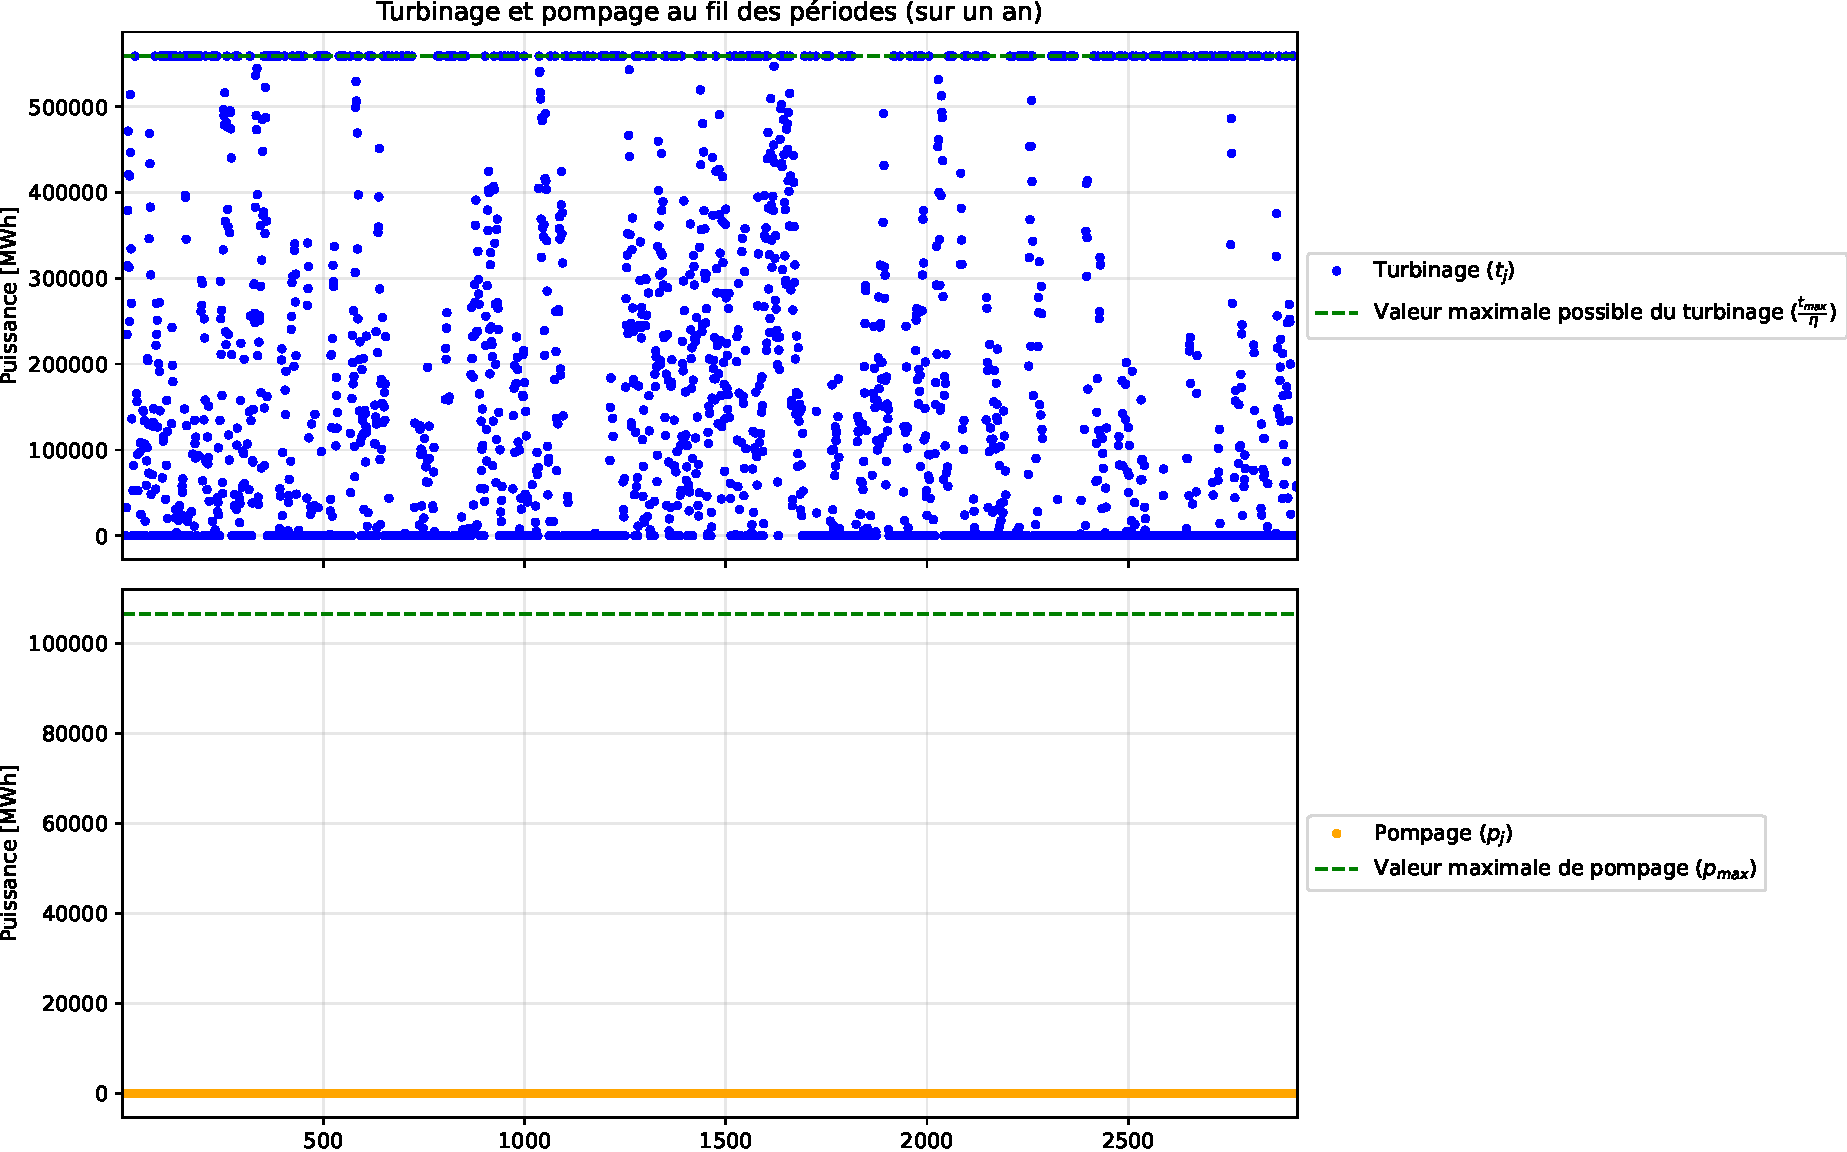
\includegraphics[scale=0.6]{GraphesP2/Turbinage_pompage_Q4.pdf}
    \caption{Représentation graphique du turbinage, du pompage, ainsi que de l'afflux naturel (en MWh stocké)
    influençant le niveau du bassin \eqref{eq:4A_contr2} pour le modèle de la question 4 par période de T = 3 heures sur un an.}
    \label{fig:Turbinage_pompage_Q4}
\end{figure}
\newpage
\begin{figure}[h!]
    \centering
    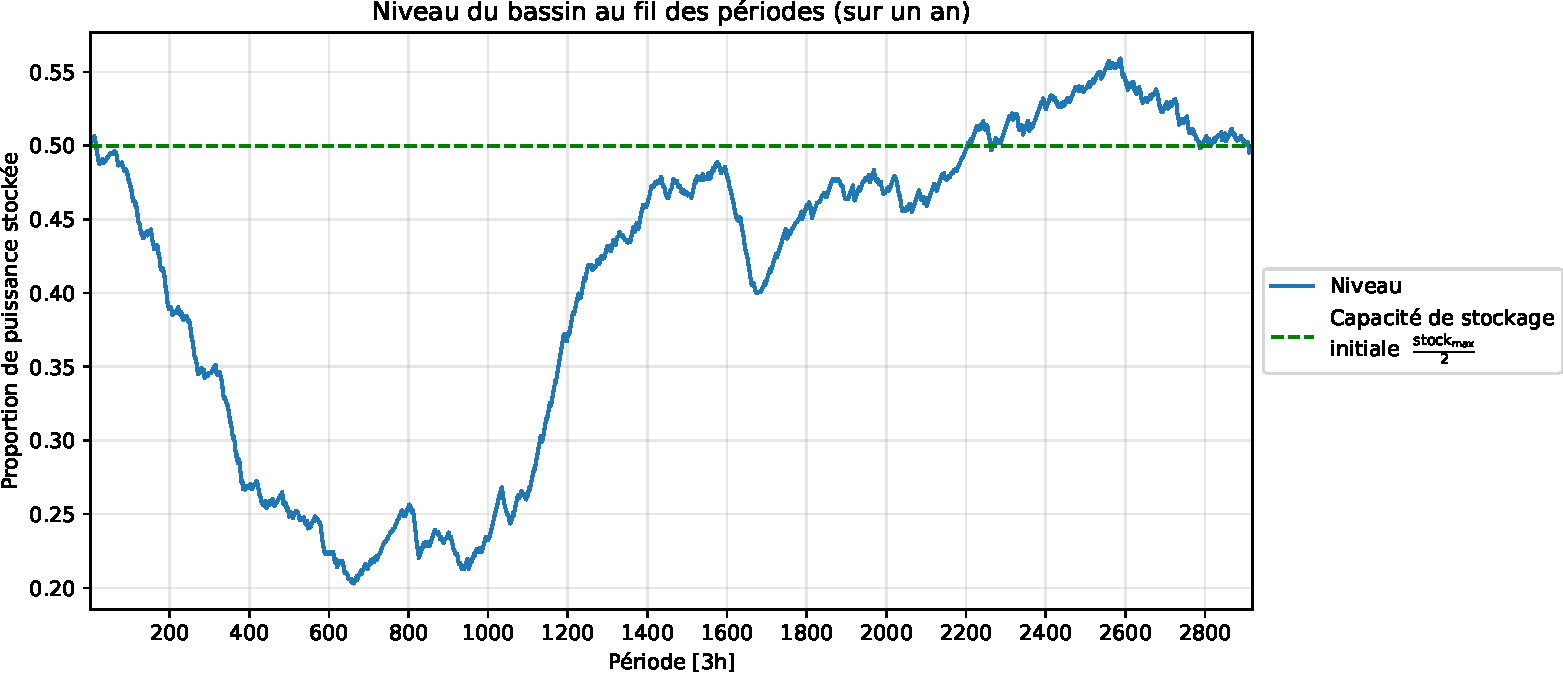
\includegraphics[scale=0.6]{GraphesP2/Niveau_Bassin_Q4.pdf}
    \caption{Représentation graphique du niveau du bassin \eqref{eq:4A_contr2} pour le modèle 
    de la question 4 par période de T = 3 heures sur un an.}
    \label{fig:Niveau_bassin_Q4}
\end{figure}
Le graphique indique bien que nous remontons au niveau initial à la fin de l'année.
\begin{figure}[h!]
    \centering
    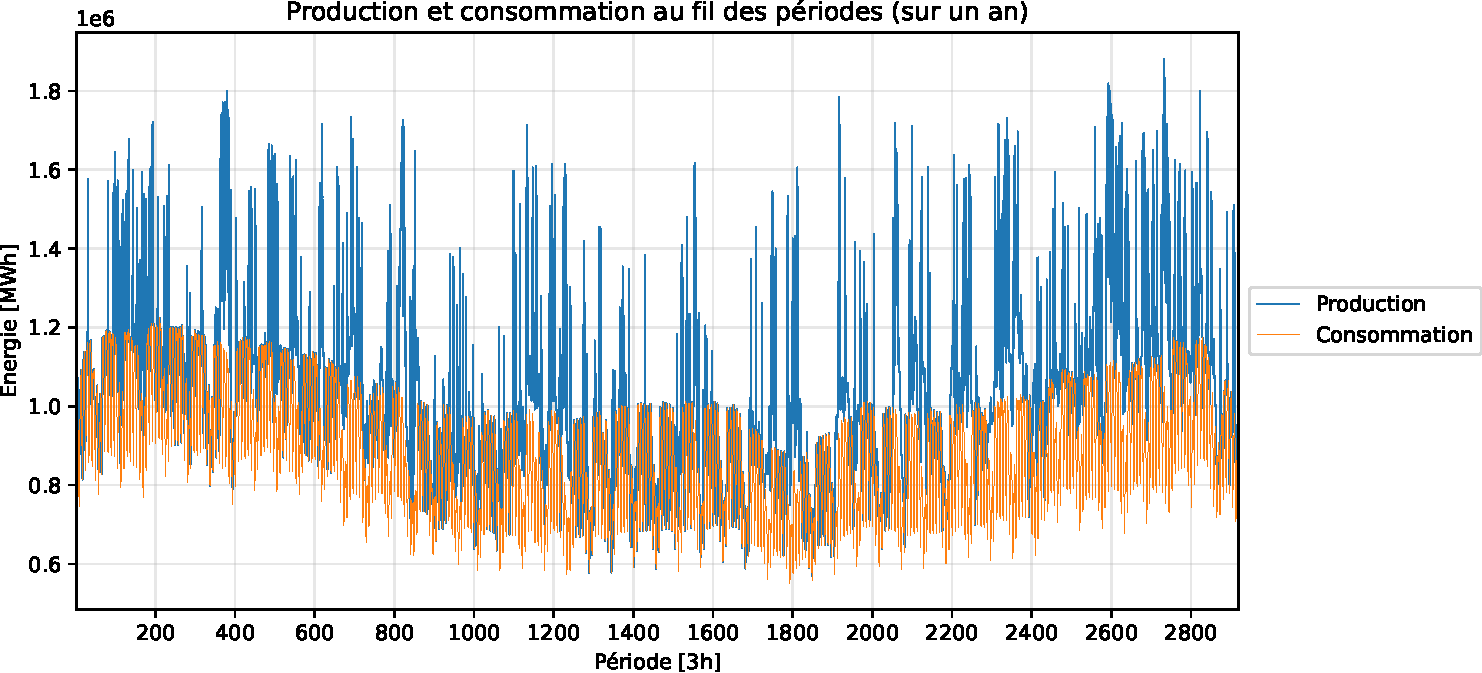
\includegraphics[scale=0.6]{GraphesP2/Prod_Cons_Q4.pdf}
    \caption{Représentation graphique de la production et de la consommation (en MWh) \eqref{eq:4A_contr1} pour le modèle de la question 4 
    par période de T = 3 heures sur un an.}
    \label{fig:Prod_Cons_Q4}
\end{figure}
Nous pouvons voir quelques écarts significatifs entre la production et la consommation, c'est-à-dire qu'à certains moments, nous gaspillons 
de l'énergie car nous produisons trop (où nous avons bien retiré à la production l'énergie stockée dans le bassin, donc il s'agit d'une perte sèche).


\clearpage
\section*{Question 4C}

\newpage
\section*{Question 5}
Nous devons à présent choisir, pour chaque site d'éoliennes, si nous installons $0\%, 50\%$ ou $100\%$ de la capacité maximale installable sur ce site.
Pour ce faire, nous rédéfinissons les variables $c_i$ de la question 4 :

\begin{table}[h!]
    \centering
    \renewcommand{\arraystretch}{1.5}% Add spacing between rows : default value is 1
    \begin{tabular}{|c || c |} 
        \hline
        Nom & Signification\\
        \hline\hline
        $c_{i} \in \{ 0, 1, 2 \}$ & Proportion de la capacité maximale $c_i^\mathrm{max}$ installée sur le i\textsuperscript{ème} site\\
        $t_j$ & Puissance à envoyer en turbinage choisie durant la j\textsuperscript{ème} période\\
        $p_j$ & Puissance de pompage choisie durant la j\textsuperscript{ème} période\\
        \hline
    \end{tabular}
    \caption{Table des nouvelles notations des variables de décisions utilisées pour le modèle de la question 5.}
    \label{table:notations_variables_5}
\end{table} 

\noindent La puissance installée sur le i\textsuperscript{ème} site équivaut alors à $0.5 \cdot c_ic_i^\mathrm{max}$. Le modèle devient alors :
\begin{align}
    \min_{c_{i} \in \mathbb{Z},t_j,p_j} \quad &\mathrm{costs}^\intercal 
    \begin{pmatrix}
        0.5 \cdot c_0c_0^\mathrm{max}\\
        \vdots\\
        0.5 \cdot c_{n-1}c_{n-1}^\mathrm{max}
    \end{pmatrix} \nonumber\\
    \textrm{tel que} \quad & \sum_{i=0}^{n-1} 0.5 \cdot c_ic_i^{max} e_i(j) + \eta \cdot t_j - p_j \ge \mathrm{cons}_j \quad \forall j \in  \{ 0, \ldots, m-1 \}\label{eq:5_contr1}\\
    & 0 \le \frac{\mathrm{stock}_\mathrm{max}}{2}  + \sum_{j=0}^{k} p_j - t_j + a_j \le  \mathrm{stock}_\mathrm{max} \quad \forall k \in \{ 0, \ldots, m-2 \}\label{eq:5_contr2}\\
    & \sum_{j=0}^{m-1} p_j - t_j + a_j = 0 \label{eq:5_contr3}\\
    & 0\le c_i \le 2 \quad \forall i \in  \{ 0, \ldots, n-1 \} \label{eq:5_contr4}  \\
    & 0 \le \eta \cdot t_j \le  t_\mathrm{max} \quad \forall j \in  \{ 0, \ldots, m-1 \} \label{eq:5_contr5}\\
    & 0 \le p_j \le  p_\mathrm{max} \quad \forall j \in  \{ 0, \ldots, m-1 \} \label{eq:5_contr6} 
\end{align}
Ici, nous avons gardé les mêmes contraintes sauf pour celles concernant les $c_i$, la \eqref{eq:5_contr4} nous dit bien
que les $c_i$ sont entre 0 et 2, et vu qu'ils sont entiers, nous avons bien nos valeurs atetndues, ensuite la \eqref{eq:5_contr1}
nous donne la même contrainte par rapport au fait que la consommation doit être satisfaite, sauf qu'il faut ajuster
les $c_i$ pour qu'ils nous donnent 0, 50\% et 100\% de la capacité maximale. Il y a également eu un léger changement dans la 
fonction objectif. \\
Pour la résolution de ce modèle, nous avons dû réduire la durée étudiée, en effet, nous avons tout d'abord
testé avec 2920 périodes (au complet), avec le solver par défaut de CVXPY, nous avions dépassé les 180 minutes
d'exécution et avons alors arrêté, ensuite nous avons testé avec le solver SCIPY et avons arrêté au-dessus de 120
minutes, nous avons en premier lieu ensuite réduit le nombre de périodes à 1500, nous avions excédé les 65
minutes avec encore le solver SCIPY. Enfin, nous avons défini le nombre de périodes à \textbf{1000}, et nous arrivons
à \textbf{46 minutes et 10.5 secondes} de calcul, donc nous avons conclu que notre choix de durée était raisonnable.
Lorsque nous résolvons notre modèle avec SCIPY pour 1000 périodes, nous obtenons un coût total de "$125.935.889.457,89$ \euro", mais il reste
à déterminer quelle est la bonne unité, en sachant que nos $c_i^{max}$ sont en $MW$, si nos coûts d'installations peuvent être amortis sur une sous-période, chose très improbable, nous aurions
alors des $\frac{\text{\euro}}{MW \cdot 1000 p}$ (en notant 1000 p le fait que nous avons 1000 périodes et en sachant 
qu'un an = 2920 p)
ce qui nous ferait un coût moyen, en divisant par la consommation sur ces 1000 périodes 
de $131.15 \frac{\text{\euro}}{MWh}$, mais ça ne semble pas être la bonne piste, gardons l'idée de l'amortissement par an, 
nous avons alors un coût total de $125.935.889.457,89 \frac{\text{\euro}}{an}$, si nous divisons par la consommation 
nous avons alors un coût moyen de $131.15 \frac{\text{\euro}}{an}*\frac{1000 p}{ MW}$, 
et si nous souhaitons des $\frac{\text{\euro}}{MWh}$, il suffit 
de multiplier par $an/ 1000 p  = \frac{2920}{1000}$ ce qui nous donne approximativement $\mathbf{382.96} \frac{\text{\euro}}{MWh}$.
Ce coût moyen est bien plus élevé que pour le modèle de la question 4, le temps de calcul a été aussi lourdement impacté, l'optimisation
par la présence des nombres entiers est bien plus complexe, et dans ce cas-ci nous amène un moins bon coût, cela s'explique par le fait qu'il
y a peu de marge sur l'ajustement des sites éoliens, et que le maximum que le solver peut faire c'est d'osciller entre 3 valeurs tout en utilisant
les capacités du bassin le mieux possible.

\begin{figure}[h!]
    \centering
    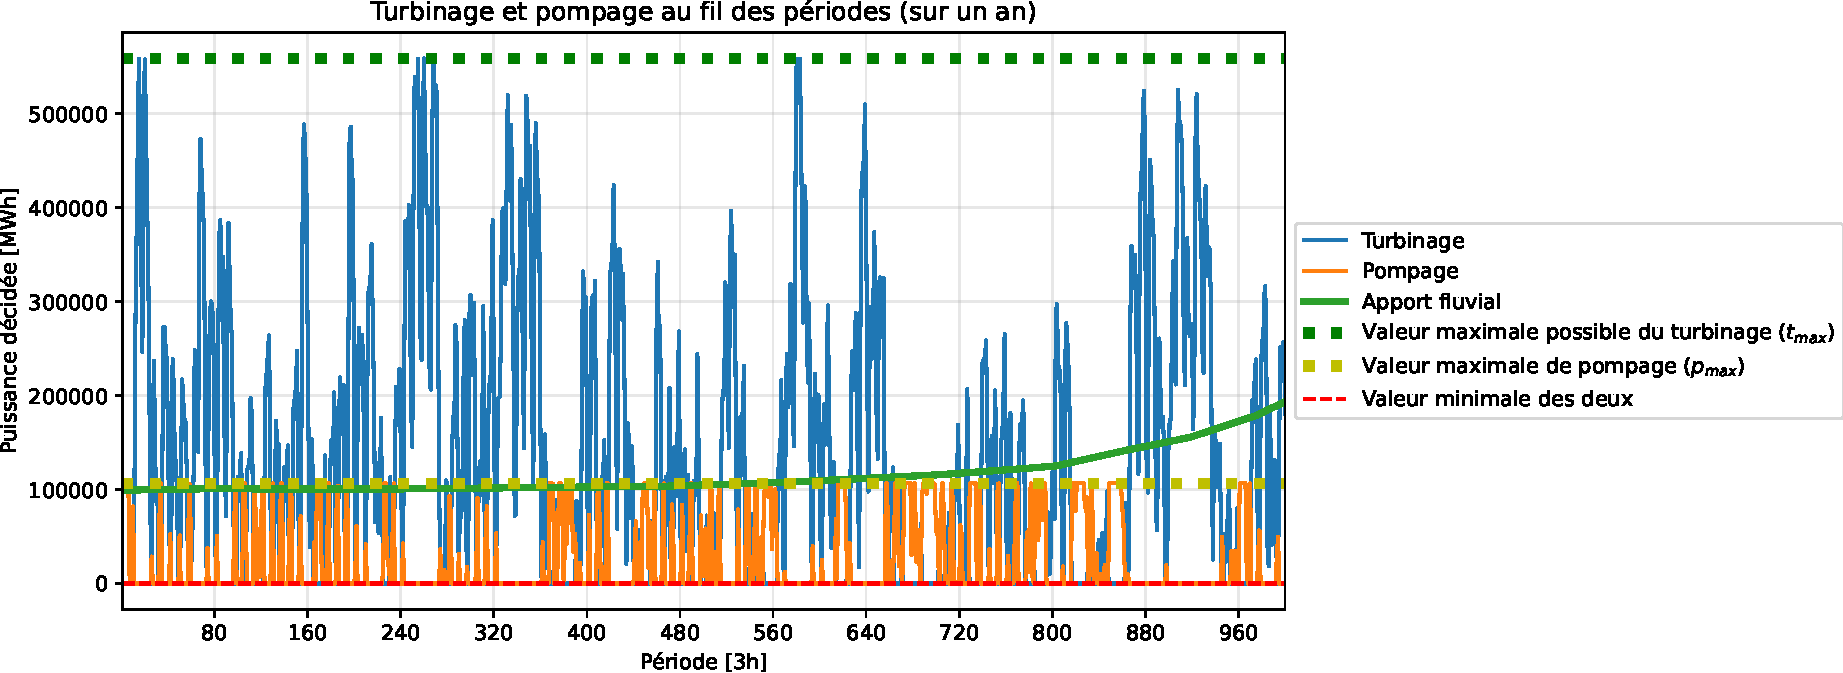
\includegraphics[scale=0.6]{GraphesP2/Turbinage_pompage_Q5.pdf}
    \caption{Représentation graphique du turbinage, du pompage, ainsi que de l'afflux naturel (en MWh stocké)
    influençant le niveau du bassin \eqref{eq:5_contr2} pour le modèle de la question 4 par période de T = 3 heures sur 1000 périodes.}
    \label{fig:Turbinage_pompage_Q5}
\end{figure}
Dans ce graphique, nous pouvons voir qu'il y a une division moins nette entre le turbinage et le pompage que dans la résolution du modèle 4, bien entendu
nous n'avons pas utilisé le même solver, mais l'impact du changement de variable de décision n'est pas négligable.

\begin{figure}[h!]
    \centering
    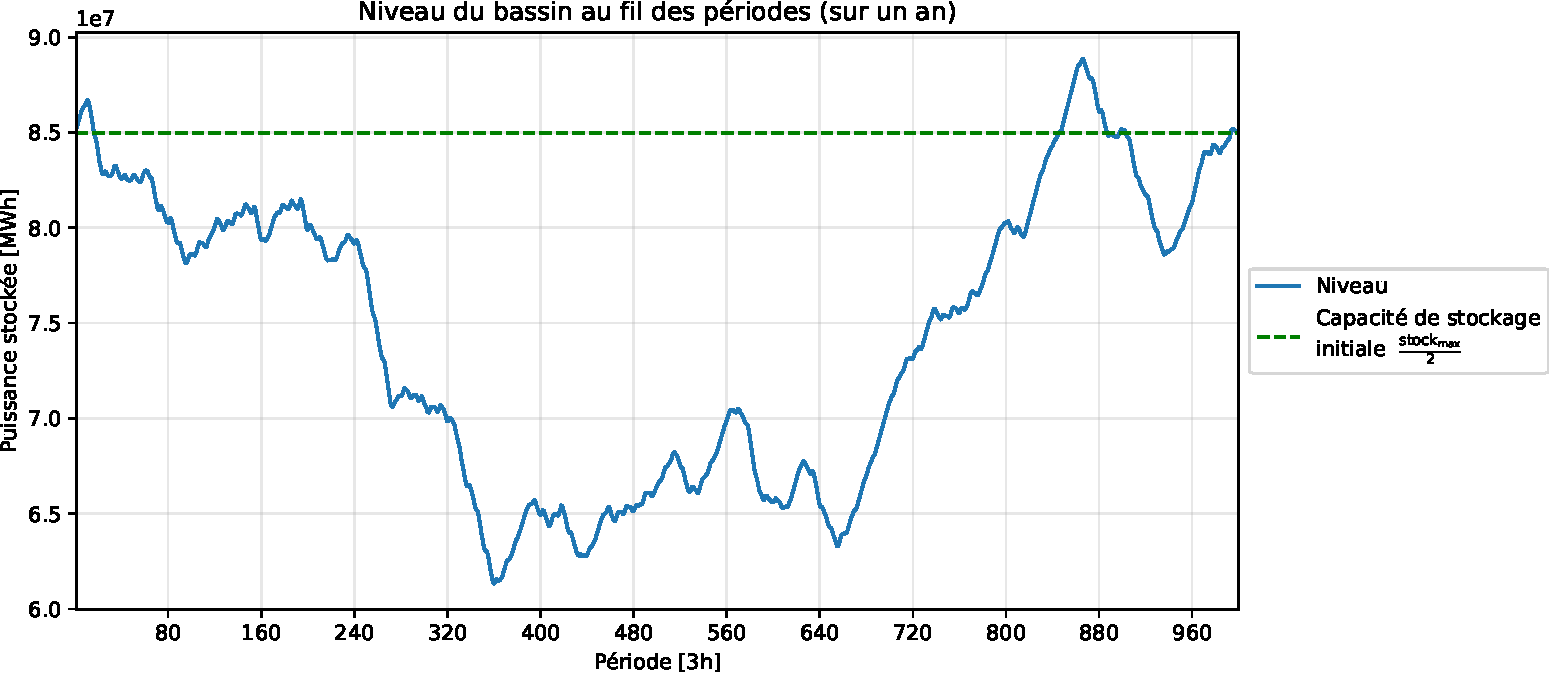
\includegraphics[scale=0.6]{GraphesP2/Niveau_Bassin_Q5.pdf}
    \caption{Représentation graphique du niveau du bassin \eqref{eq:5_contr2} pour le modèle 
    de la question 5 par période de T = 3 heures sur 1000 périodes.}
    \label{fig:Niveau_bassin_Q5}
\end{figure}
Le graphique indique bien que nous remontons au niveau initial à la fin de la période.
\newpage
\begin{figure}[h!]
    \centering
    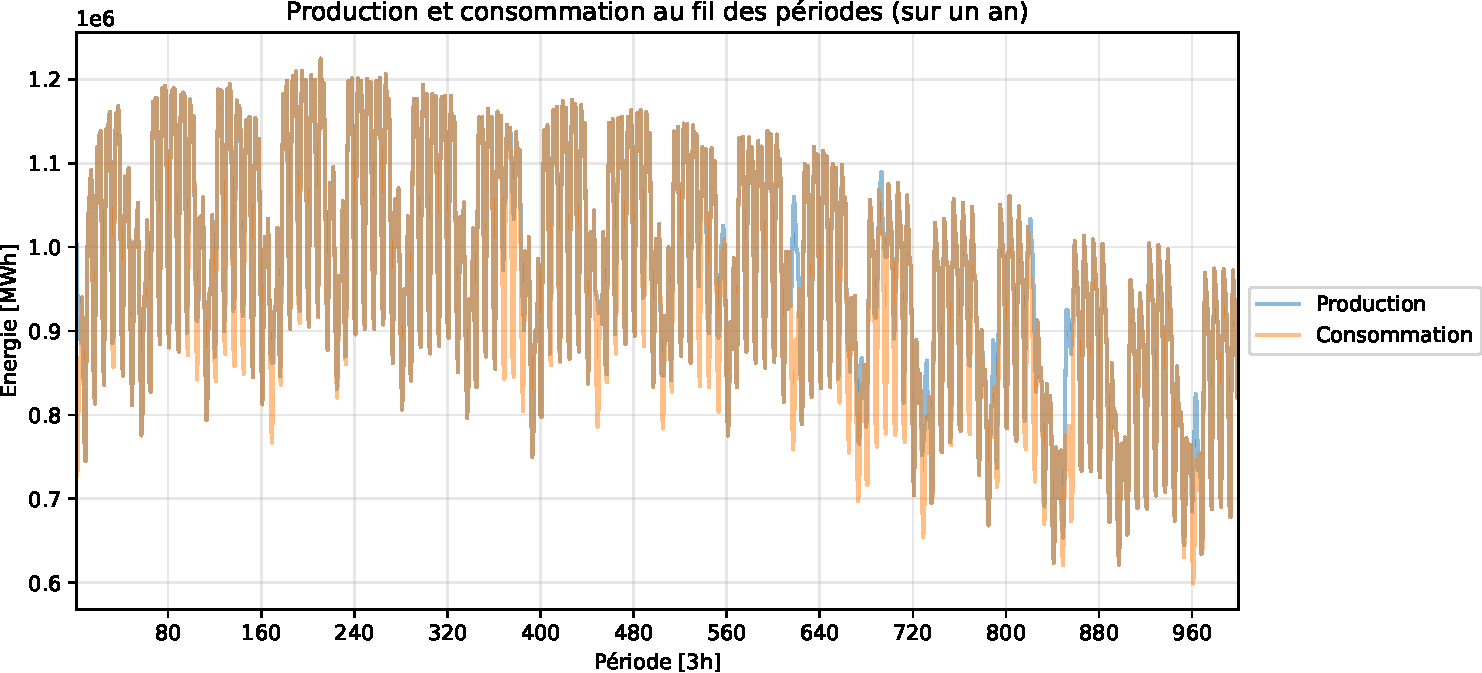
\includegraphics[scale=0.6]{GraphesP2/Prod_Cons_Q5.pdf}
    \caption{Représentation graphique de la production et de la consommation (en MWh) 
    \eqref{eq:5_contr1} pour le modèle de la question 5 par période de T = 3 heures sur 1000 périodes.}
    \label{fig:Prod_Cons_Q5}
\end{figure}
Dans ce graphique, la production est beaucoup plus proche de la consommation par rapport à la question précédente, nous sommes certainement dans cette solution
obligé d'aller puiser au maximum pour éviter le gaspillage d'un surplus de production.
\noindent 


\end{document}
